\subsection{Balanço de Massa}

O balanço de massa aplica o princípio da conservação da massa a sistemas de processo: em regime estacionário, a massa que entra em um sistema deve ser igual à massa que sai, ajustada pela geração ou consumo devido a reações químicas \cite{felder2005}. Para cada componente, a quantidade produzida ou consumida deve ser contabilizada segundo a estequiometria.

A Tabela \ref{tab:unidades-balanco-massa} resume a base dimensional comum das Equações \ref{eq:mass_balance_word} a \ref{eq:gross_product_flow}. A mesma base deve ser mantida dentro de cada balanço.

\begin{table}[H]
    \centering
    \caption{Unidades e natureza dos termos no balanço de massa com reciclo}
    \label{tab:unidades-balanco-massa}
    \begin{tabular}{|p{0.30\textwidth}|p{0.60\textwidth}|}
        \hline
        \textbf{Símbolo ou termo} & \textbf{Unidade ou natureza} \\ \hline
        Acúmulo, entradas, saídas, geração e consumo & Mesma base escolhida para o balanço por tempo, como $\mathrm{kg/s}$ ou $\mathrm{mol/s}$. \\ \hline
        $\dot{m}$ & Vazão mássica, por exemplo $\mathrm{kg/s}$. \\ \hline
        $F_R$, $F_G$, $F_P$ & Vazões na mesma base selecionada para o balanço: molar, mássica ou volumétrica. \\ \hline
        $f$ & Fração de reciclo ou purga adimensional. \\ \hline
    \end{tabular}
\end{table}

\begin{equation}
\text{Acúmulo} = \text{Entradas} - \text{Saídas} + \text{Geração} - \text{Consumo}
\label{eq:mass_balance_word}
\end{equation}

No estado estacionário sem reação, o acúmulo é zero, de modo que:

\begin{equation}
\sum \dot{m}_{\mathrm{entrada}} = \sum \dot{m}_{\mathrm{saida}}
\label{eq:steady_state_mass_balance}
\end{equation}

Por componente $i$, incluindo reação química:

\begin{equation}
\sum \left(\dot{m}_{\mathrm{entrada},i} + \dot{m}_{\mathrm{geracao},i}\right) = \sum \left(\dot{m}_{\mathrm{saida},i} + \dot{m}_{\mathrm{consumo},i}\right)
\label{eq:component_mass_balance_rxn}
\end{equation}

Em problemas industriais, frequentemente há reciclo e purgas envolvidos nos balanços. Nesses casos, para divisores de fluxo (\textit{splitters}), define-se por exemplo:

\begin{equation}
F_{R} = f \cdot F_{P}
\label{eq:recycle_flow}
\end{equation}

\begin{equation}
F_{G} = ( 1 - f ) \cdot F_{P}
\label{eq:gross_product_flow}
\end{equation}

Esses parâmetros permitem fechar balanços em sistemas com recirculação e calcular a acumulação de inertes ou subprodutos. Na Figura \ref{fig:mass_balance_results}, é apresentado o resultado gerado pelo \textit{software} para um balanço de massa contendo reciclo e reação.

\begin{figure}[H]
    \centering
    \caption{Resultados do balanço de massa com reciclo e reação}
    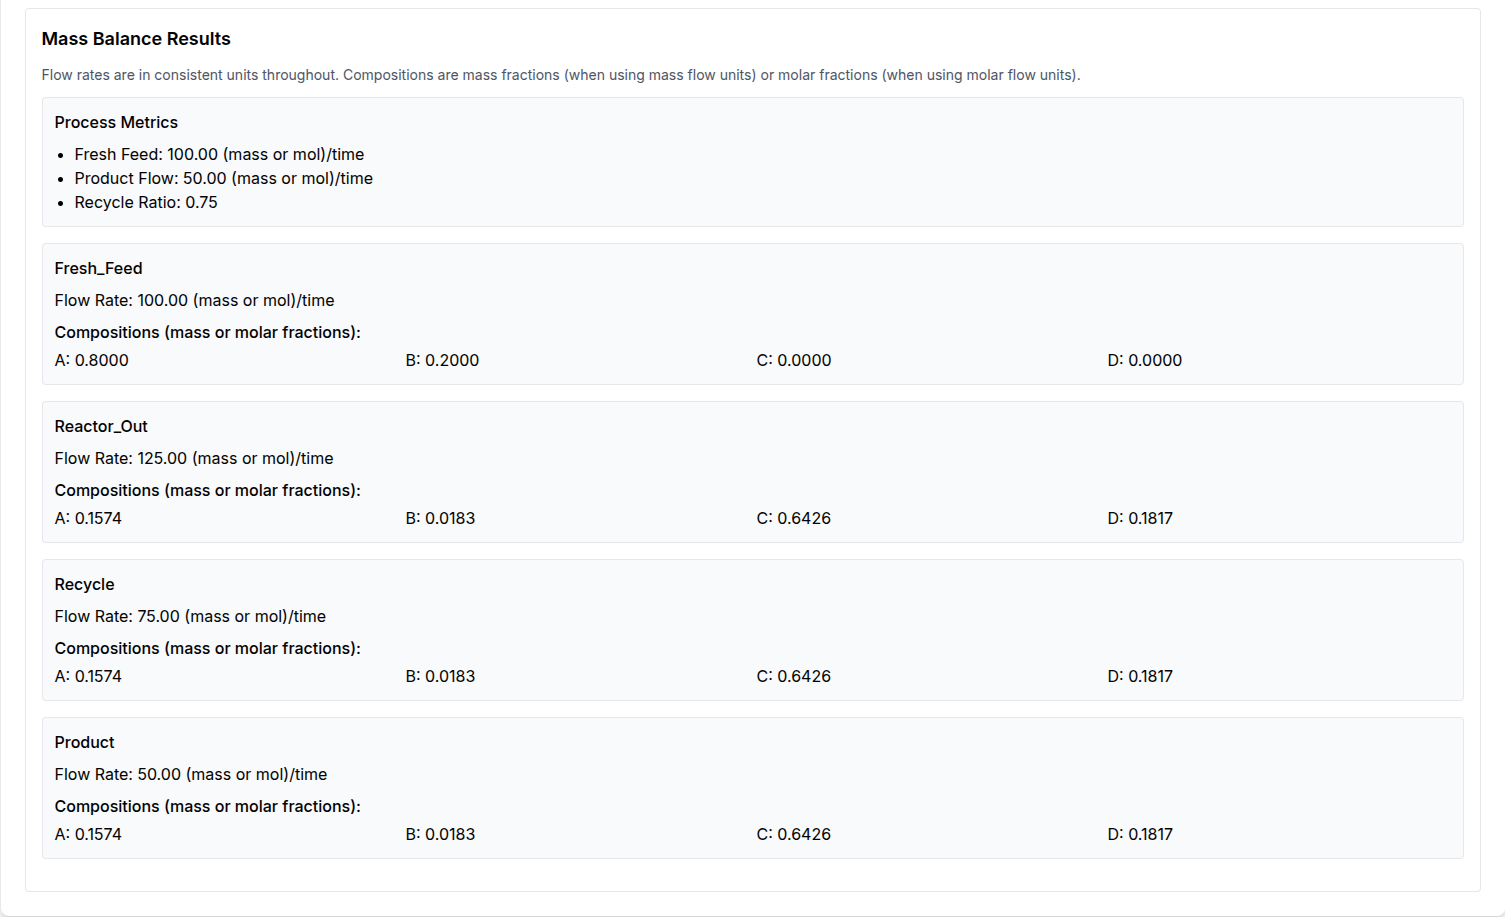
\includegraphics[width=\linewidth]{media/cap4_resultados_balanco_massa_reacao_reciclo.png}
    \fonte{Elaboração própria (2026).}
    \label{fig:mass_balance_results}
\end{figure}

O balanço de massa fundamenta o dimensionamento de equipamentos como misturadores, separadores, reatores e redes de processo, além de embasar análises econômicas (minimizando perdas de matérias-primas) e de segurança (evitando acúmulo indesejado de compostos). Vale notar que temperatura e pressão influenciam o balanço apenas através de propriedades físicas (massa específica, volumes específicos), ou mudanças de fase que afetem as vazões mássicas e molares de cada corrente \cite{felder2005}.
